% !TEX encoding = UTF-8 Unicode
\documentclass[a4paper]{article}

\usepackage{color}
\usepackage{url}
\usepackage[T2A]{fontenc} % enable Cyrillic fonts
\usepackage[utf8]{inputenc} % make weird characters work
\usepackage{graphicx}
\usepackage{amsmath}

\usepackage[english,serbian]{babel}
%\usepackage[english,serbianc]{babel} %ukljuciti babel sa ovim opcijama, umesto gornjim, ukoliko se koristi cirilica

\usepackage[unicode]{hyperref}
\hypersetup{colorlinks,citecolor=green,filecolor=green,linkcolor=blue,urlcolor=blue}

\usepackage{listings}

%\newtheorem{primer}{Пример}[section] %ćirilični primer
\newtheorem{primer}{Primer}[section]

\definecolor{mygreen}{rgb}{0,0.6,0}
\definecolor{mygray}{rgb}{0.5,0.5,0.5}
\definecolor{mymauve}{rgb}{0.58,0,0.82}

\lstset{ 
  backgroundcolor=\color{white},   % choose the background color; you must add \usepackage{color} or \usepackage{xcolor}; should come as last argument
  basicstyle=\scriptsize\ttfamily,        % the size of the fonts that are used for the code
  breakatwhitespace=false,         % sets if automatic breaks should only happen at whitespace
  breaklines=true,                 % sets automatic line breaking
  captionpos=b,                    % sets the caption-position to bottom
  commentstyle=\color{mygreen},    % comment style
  deletekeywords={...},            % if you want to delete keywords from the given language
  escapeinside={\%*}{*)},          % if you want to add LaTeX within your code
  extendedchars=true,              % lets you use non-ASCII characters; for 8-bits encodings only, does not work with UTF-8
  firstnumber=1000,                % start line enumeration with line 1000
  frame=single,	                   % adds a frame around the code
  keepspaces=true,                 % keeps spaces in text, useful for keeping indentation of code (possibly needs columns=flexible)
  keywordstyle=\color{blue},       % keyword style
  language=Python,                 % the language of the code
  morekeywords={*,...},            % if you want to add more keywords to the set
  numbers=left,                    % where to put the line-numbers; possible values are (none, left, right)
  numbersep=5pt,                   % how far the line-numbers are from the code
  numberstyle=\tiny\color{mygray}, % the style that is used for the line-numbers
  rulecolor=\color{black},         % if not set, the frame-color may be changed on line-breaks within not-black text (e.g. comments (green here))
  showspaces=false,                % show spaces everywhere adding particular underscores; it overrides 'showstringspaces'
  showstringspaces=false,          % underline spaces within strings only
  showtabs=false,                  % show tabs within strings adding particular underscores
  stepnumber=2,                    % the step between two line-numbers. If it's 1, each line will be numbered
  stringstyle=\color{mymauve},     % string literal style
  tabsize=2,	                   % sets default tabsize to 2 spaces
  title=\lstname                   % show the filename of files included with \lstinputlisting; also try caption instead of title
}

\begin{document}

\title{Naslov seminarskog rada\\ \small{Seminarski rad u okviru kursa\\Metodologija stručnog i naučnog rada\\ Matematički fakultet}}

\author{Aleksandra Bošković, Stefan Jaćović,Milena Stojić, četvrti autor\\ kontakt email aleksandra94@hotmail.rs, stefanjacovic25@gmail.com,mstojic39@yahoo.com, četvrtog autora}

%\date{9.~april 2015.}

\maketitle

\abstract{
U ovom tekstu je ukratko prikazana osnovna forma seminarskog rada. Obratite pažnju da je pored ove .pdf datoteke, u prilogu i odgovarajuća .tex datoteka, kao i .bib datoteka korišćena za generisanje literature. Na prvoj strani seminarskog rada su naslov, apstrakt i sadržaj, i to sve mora da stane na prvu stranu! Kako bi Vaš seminarski zadovoljio standarde i očekivanja, koristite uputstva i materijale sa predavanja na temu pisanja seminarskih radova. Ovo je samo šablon koji se odnosi na fizički izgled seminarskog rada (šablon koji \emph{morate} da koristite!) kao i par tehničkih pomoćnih uputstava. Pročitajte tekst pažljivo jer on sadrži i važne informacije vezane za zahteve obima i karakteristika seminarskog rada.}

\tableofcontents

\newpage

\section{Uvod}
\label{sec:uvod}

Simulirano kaljenje (Simulated Annealing, SA) je metoda zasnovana na lokalnom pretraživanju, uz mehanizam inspirisan procesom kaljenja čelika koji omogućava izlazak iz lokalnog optimuma. Algoritam je predložen 1983. godine od strane Kirkpatrika i drugih.
Pri procesu metalurškog kaljenja čelika cilj je oplemenjivanje metala tako da on postane čvršći. Da bi se postigla čvrstoća metala potrebno je njegovu kristalnu rešetku pomeriti tako da ima minimalnu potencijalnu energiju. Prvi korak u kaljenju čelika je zagrevanje do
određene visoke temperature, a zatim nakon kratkog zadržavanja na toj temperaturu počinje postepeno hlađenje. Pri postepenom hlađenju atomi metala nakon procesa kaljenja formiraju
pravilnu kristalnu rešetku i time se postiže energetski minimum kristalne rešetke. Važno je napomenuti da brzo hlađenje može da uzrokuje pucanje metala.

\begin{figure}[h!]
\centering
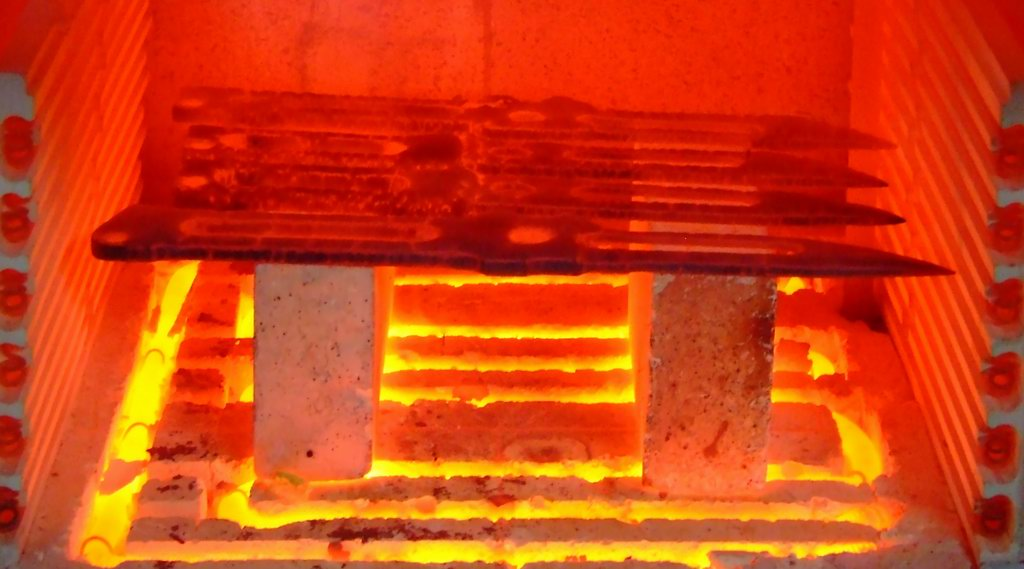
\includegraphics[scale=0.3]{kal.jpg}
\caption{Kaljenje čelika}
\label{fig:universe}
\end{figure}

Funkcija cilja za koju se traži globalni optimum se može posmatrati kao energija kristalne rešetke ako je potrebno minimizovati funkciju cilja ili negativna energija kristalne rešetke ako
je potrebno maksimizovati funkciju cilja. Metoda počinje izborom početnog rešenja i postavljanjem početne temperature na relativno visoku vrednost. Zatim se na slučajan način bira
jedno rešenje iz okoline tekućeg rešenja. Ako je to rešenje bolje, onda ono postaje novo tekuće rešenje. Ako je novo rešenje lošije od tekućeg, ono ipak može da postane tekuće rešenje, ali
sa određenom verovatnoćom. Verovatnoća prihvatanja lošijeg rešenja obično zavisi od parametra koji predstavlja temperaturu i vremenom opada kako se algoritam izvršava. Ovakav pristup obezbeđuje izlazak iz lokalnog optimuma. U početku je ta verovatnoća velika, pa će
u cilju prevažilaženja lokalnog optimuma lošije rešenje biti prihvaćeno. Pred kraj izvršavanja
algoritma verovatnoća prihvatanja lošijeg rešenja je jako mala i to se verovatno neće ni desiti,
jer se smatra da je optimum dostignut ili se nalazi blizu najboljeg posećenog rešenja, pa se
izbegava pogoršanje tekućeg rešenja.


\section{Algoritam}
Ideja implementacije algoritma simuliranog kaljenja je sledeca.U svakoj iteraciji algotitma primenjenog na diskretan problem poredimo dve vrednosti resenja, trenutno najbolje i novo generisano resenje. Zavisno od uslova odabira izmedju ova dva resenja za narednu iteraciju dobijeno resenje prelazi u sledecu iteraciju. Proces ponavljamo  dok god se ne zadovolji uslov zaustavljanja. Uslov zaustavljanja moze biti zadat konacnim brojem iteracija ili dok se ne dostigne trazeni minimum(maximum).

\subsection{Definisanje termina}
Da bismo opisali specifičnosti algoritma simuliranog kaljenja uvedimo nekoliko pojmova koji ce nam biti potrebni za razumevanje samog algoritma.Neka je $\Omega$ prostor mogucih resenja,$f:\Omega \rightarrow \Re$ funkcija definisana nad prostorom $\Omega$. Cilj je pronaci  $w\in\Omega$ za koje funkcija $f$ doseze minimum(maksimum) problema na koji primenjujemo algoritam simuliranog kaljenja.Ukoliko postoji $w*\in\Omega$ za koje  vazi:$$f(w*)\geq f(w) , \forall w \in \Omega$$ tada je $w*$ trazeni maximum.Da bi ovakvo $w$ postojalo neophodan uslov je da funkcija $f$ bude ogranicena na prostoru $\Omega$.Definisimo i funkciju $N(w)$ pomocu koje cemo odredjivati susedna resenja resenju  $w\in\Omega$ u svakoj iteraciji algoritma pretrage novog resenja. \par

\subsection{Odabir resenja}
Neka je $w\in\Omega$ inicijalno resenje problema koje proizvoljno biramo iz skupa $\Omega$ i $w'\in N(w)$ proizvoljno odabrano susedno resenje nekim predefinisanim prailom ili slucajnim izborom. Ukoliko pogledamo uslov da resenje bude maximum zakljucujemo da nam je bolje ono resenje koje ima vecu vrednost funkcije $f$.Ukoliko bismo u svakoj iteraciji birali resenje koje ima vecu vrednost funkcije $f$ algoritam bi se sveo na algoritam penjanja uzbrdo.Problem algoritma penjanja uzbrdo se javlja kada se naidje na lokalni maximum i tu se dalja pretraga zaglavljuje jer svako susedno resenje nije bolje od njega.Jos jedna situacija u kojoj algoritam penjanja uzbrdo pokazuje slabosti je pojava platoa gde iz istog razloga pretraga ostane zaglavljena.Da bismo resili ovakve probleme algoritam simuliranog kaljenja za odluku koje od dva resenja ce uzeti za sledecu iteraciju bazira na verovatnoci $p$ prihvatljivosti da novo resenje bude uzeto za trenutno u narednoj iteraciji.
\[ p =
  \begin{cases}
    \exp(f(w')-f(w)/t_k)  \quad f(w) > f(w'),\\
    1  \quad f(w) \leq f(w')\\
  \end{cases}
\]


gde je $t_k$ temperaturni parametar iteracije k i n maximali broj iteracija za koji vazi:
$$\forall k\leq n, \quad t_k > 0 \quad \lim_{k \to \infty}t_k=0 $$

\subsection{Imlementacija algoritma}
\textbf{Ulaz:} Inicijalno resenje $w$,pocetna vrednost $t_k$ kao i vrednost $M_k$ koja predstavlja koliko puta ponavljati iteraciju sa datom vrednoscu $t_k$
 \par
\textbf{Izlaz:} $w$ najbolje resenje datog problema koje je algoritam uspeo da pronadje
\newline
Ponavljaj:
\begin{itemize}
\item[] $m=0$
\item[]  Ponavljaj:
\begin{itemize}
\item[] generisi novo resenje  $w'\in N(w)$
\item[] izracunaj vrednost  $\Delta=f(w')-f(w)$
\item[] ako je $\Delta \geq 0$
\begin{itemize}
\item[] $w=w'$ 
\end{itemize}
\item[]inace
\begin{itemize}
\item[] sa verovatnocom $p=\exp(-\Delta/t_k)$ vazi $w=w'$ 
\end{itemize}
\item[]$m=m+1$
\end{itemize}
\item[]dok ne bude $ m=M_k$
\item[] $k=k+1$
\end{itemize}
Dok god nije zadovoljen uslov zaustavljanja


\subsection{Primena algoritma simuliranog kaljenja na problem trgovackog putnika}


	Problem trgovackog putnika je jedan od najizucavanijih kombinatornih problema kao i NP problema.Problem je definisan sa sledeci nacin.
	Data nam je lista gradova koje putnik treba da obidje i da se vrati u grad iz kog je krenuo.Takoje potreban podatak nam je koja je udajenost izmedju svaka dva grada iz liste gradova.Nas zadatak je da pronadjemo redosed obilaska gradova tako da ukupna duzina puta koji putnik treba da predje bude minimalna.\par
	Prvo resenje koje se namece je agoritam grube sile,a to je ispitivanje svih mogucih nacina obilazaka gradova i odabir najbolje kombinacije za koju je ukupna duzina minimalna.Ovakvo resenje nije isplativo zbog velike vremenske slozenosti koja iznosi n! pri cemu je n broj gradovi koje putnik treba da poseti.\par
    
Da bi problem resili algoritmom simuliranog kaljenja definisimo prvo sta nam predstavlja temperatura iz ovog algoritma. Temperatura kod ovog problema predstavljala bi meru slucajnosti promene putanje pri cemu se trazi najmanja putanja. Ukoliko je vrednost temperature visoka prave se i vece slucajne promene i pritom se izbegava rizik da ostanemo zaglavljeni u lokalnom optimumu, a njih ima mnogo u posmatranom problemu.Kako temperatura pada tako se spustamo u skoro optimalni minimum. U svakom koraku kada je potrebna promena temperature njena vrednost je 0.9 puta veca od prethodne. Ovim zadovoljavamo uslov da pad temperature tezi nuli kroz rast broja iteracija.\par

Proces kaljenja pocinje stazom koja jednostavno navodi sve gradove redosledom njihovog odabira za obilazak. Na svakom temperaturnom koraku se vrsi odredjeni broj slucajnih transformacija puta.Nacin transformacije puta moze biti razlicit.Moguce je izabrati dva grada i zameniti njihovo mesto u redosledu obilaska gradova, drugi od nacina bio bi odabrati dve pozicje koje oznacavaju segment koji ce se prebaciti na odredjeno mesto u stazi koja predstavlja redosled obilaska, ili dati segment rotirati. Ukoliko zelimo da se vrsi vise nacina transformacija uvodimo "softverski novcic" koji bi odredjivao vrstu transformacije. 
 Duzina modifikovanog puta se zatim izracunava i uporedjuje sa stazom pre modifikacije, stvarajuci velicinu koju nazivamo razliku u troskovima. Ako je ta velicina negativna, onda modifikovana puranja je kraca od originalne putanje i uvek je zamenjuje. Medjutim, ako dodje do povecanja troskova, eksponencija njegove negativne velicine deljenja sa trenutnom remperaturom uporedjuje se sa jednolicno raspodeljenim slucajnim brojem izmenju 0 i 1, a ako je vece modifikovana puta ce se koristi iako je povecala troskove. U pocetku ce prihvatanje duzeg puta biti vise verovatno jer je temperatura visoka, ali kako temperatura opada bice prihvacena samo manja povecanja troskova. Broj promena koje se testiraju na svakoj temperaturi je proizvoljan, temperatura se smanjuje i pretraga nastavlja. Nakon isprobljavanja svih mogucih scenarija na odredjenoj temperaturi, nisu pronadjene promene koje smanjuju duzinu puta, resenje se smatra dovoljno dobrim i prikazuje se dobijena staza.

\begin{primer}
Neka nam je dato 5 gradova i matrica M koja predstavlja medjusobne udaljenosti izmedju gradova tako da je $M[i][j]$ udaljenost izmedju gradova $i$ i $j$. Pronaci permutaciju gradova tako da polazeci iz prvog grada se preko ostalih gradova stigne u pocetni uz uslov da je predjeni put minimalni.\par
Nacin implementacije resenja u jeziku Python prikazan je kroz listing \ref{simple}. 
\end{primer}

\begin{lstlisting}[caption={Resavanje problema TSP koriscenjem SA algoritma},frame=single, label=simple]
import numpy as np
import itertools as per
import random
import math 
M = np.array([
   [0,10,3,12,7],
   [10,0,11,7,3],
   [3,11,0,8,8],
   [12,7,8,0,1],
   [7,3,8,1,0]])
def suma (l):
  return M[l[0]][l[1]]+M[l[1]][l[2]]+M[l[2]][l[3]]+M[l[3]][l[4]]+M[l[4]][l[0]]
Oznake_gradova = np.array([0,1,2,3,4])
#Postavimo pocetnu permutaciju, tekucu duzinu puta i pocetnu temperaturu
#Pretpostavimo da racunamo jednu iteraciju za svaku temperaturu
minimum=sum(Oznake_gradova)
minimum_perm=Oznake_gradova
t=20
k=0
lista=minimum_perm

while k<25:
  nova_per = random.choices(Oznake_gradova,k=2)
  lista[nova_per[0]], lista[nova_per[1]] = lista[nova_per[1]], lista[nova_per[0]]
  s=suma(lista)
  razlika=s-minimum
  
  if razlika < 0:
    minimum=s
    per_min=lista
  else:
    p=math.exp(s-minimum/t)
    q=random.uniform(0, 1)
    if p > q :
      minimum=s
      per_min=lista
  k=k+1
  t=t*0.9
\end{lstlisting}






\section{Genetsko kaljenje}
Dve osnovne metaheuristike koje pripadaju široj grupi algoritama pretage su simulirano kaljenje i genetski algoritom.Sa idejom da se iskoriste prednosti obe metoda nastaje genetsko kaljenje.Tvorac koncepta je Kenneth Price koji je 1994 u svo clanku u casopisu "Dr.Bobbs Journal" prvi put izneo ideju o spajanju simuliranog kaljenja i genetskog algoritma. \par
Simulirano kaljenje je algoritam koji se uglavnom primenjuje kada postoji jedno optimalno resenje, dok se genetski primenjuje u slucaju postojanja vise optimalnih resenja.Ovu ideju koristimo u algoritmu genetskog kaljenja. \par
Genetski algoritam kroz iteracije evoluira ka boljim resenjima od pocetno zadatih resenja.U svakoj iteraciji neophodn je odabrati jedinke za ukrstanje i mutaciju.Algoritam genetskog kaljenja ideju simuliranog kaljenja koristi u procesu odabira jedinki.


\subsection{Prednosti i nedostaci simuliranog kaljenja}

Prednost simuliranog kaljenja (u odnosu na klasican genetski algoritam) je dobra lokalna pretraga.(c) Ono ce uvek naci najbolje resenje u neposrednoj blizini. Medjutim to je u isto vreme i slabost, iako u teoriji ovaj algoritam moze da konvergira ka globalnom optimalnom resenju. \par
Ovaj nedostatak moze da se prevazidje sa vise zasebnih izvrsavanja. Svako sledece izvrsavanje pocinjemo sa novim pocetnim resenjem. Na kraju uzimamo najbolji finalni rezultat. U narednim iteracijama ne koristimo znanje dobijeno u prethodnim iteracijama. To je mana ovog pristupa. \par
Prednost genetskog algoritma u odnosu na simulirano kaljenje je i u visestrukosti resenja. Simuliranim kaljenjem mi samo poboljsavamo jedno resenje. Bolja je pretraga zasnovana na $m$ > 1 dobrih resenja.





\section{Zaključak}
\label{sec:zakljucak}

Pojava metode simuliranog kaljenja (1983) prouzrokovala je novi pristup pri rešavanju
problema kombinatorne optimizacije i podstakla razvoj metaheurističkih algoritama. U kasnijim godinama predstavljeno je mnogo novih algoritama, najviše baziranih na prirodnim
fenomenima, kao što su metoda zasnovana na ponašanju mrava (Ant Colony Optimization –ACO), metoda zasnvana na ponašanju roja čestica (Particle Swarm Optimization –
PSO) , metoda veštačkog imuniteta (Artificial Immune System – AIS).


\addcontentsline{toc}{section}{Literatura}
\appendix
\bibliography{seminarski} 
\bibliographystyle{plain}

\appendix

\end{document}